\chapter{Theory}
\label{ch:architecture}

\section{Optical Principles and Numerical Simulation}
在這個章節中，我會詳細推導並說明光在矽基整合光學波導中的傳播物理，以及模態分波解多工器運作的理論基礎，
最後會介紹數值模擬的基礎理論。我們將從電磁場數學模型出發，分析奈米級波導的邊界條件與模態行為，
作為後續反向設計演算法與模型預測的依據。
\subsection{Waveguide Physics and Eigenmode Theory}
首先，在波導中，光會被侷限在折射率較高的矽核心中，並透過全反射(Total internal reflection, TIR)進行傳播。
關於介電質波導中電磁場行為與模態特徵值問題的完整理論架構，本節主要參考 A. Yariv 的經典著作 \cite{yariv2007_photonics} 所建立的物理模型。
在無自由電荷($\rho = 0$)且無源($\vec{J} = 0$)的介電質波導環境中，
我們可以用馬克士威方程(Maxwell equations)中的法拉第電磁感應定律\eqref{eq:maxwell1}與馬克士威-安培定律\eqref{eq:maxwell2}微分式
來描述光的傳播行為，如下所示：
\begin{align}
\nabla \times \vec{E} &= -\frac{\partial \vec{B}}{\partial t}
\label{eq:maxwell1} \\
\nabla \times \vec{H} &= \frac{\partial \vec{D}}{\partial t}
\label{eq:maxwell2}
\end{align}
這時候引入了材料的介電質($\epsilon$)和導磁率($\mu$)，假設光場在具有時諧性(Time-Harmonic)，則\eqref{eq:maxwell1}和\eqref{eq:maxwell2}
馬克士威方程可以寫成頻域複數形式:
\begin{align}
\nabla \times \vec{E} &= -i\omega\mu\vec{H}
\label{eq:freq_maxwell1} \\
\nabla \times \vec{H} &= i\omega\epsilon\vec{E}
\label{eq:freq_maxwell2}
\end{align}
接著，我們再對馬克士威方程頻域複數形式\eqref{eq:freq_maxwell1}與\eqref{eq:freq_maxwell2}取旋度，再均勻的介質中，由於$\nabla\cdot\vec{E} = 0$，
因此，我們即可推導出經典的亥姆霍茲方程(Helmholtz Equation):
\begin{align}
\nabla^2\vec{E} + k_0^2 n^2(\vec{r})\vec{E} = 0
\label{eq:helmholtz}
\end{align}
其中，$k_0 = \frac{\omega}{c}$為真空中的波數，介電常數與折射率($n$)關係為$\epsilon = n^2\epsilon_0$，
因此光子能夠被侷限在波導內部傳播，就是因為波導核心層與包層之間的折射率差而產生的全反射(TIR)，在本篇矽基波導的核心
材料為矽(Silicon, Si)，其折射率($n_{\mathrm{Si}}$)約為3.48; 而包層為二氧化矽(Silicon dioxide, $\mathrm{SiO_2}$)，
其折射率($n_{\text{SiO}_2}$)約為1.44，如圖~\ref{fig:waveguide_schematic}所示。

\begin{figure}[htb]
	\centering
	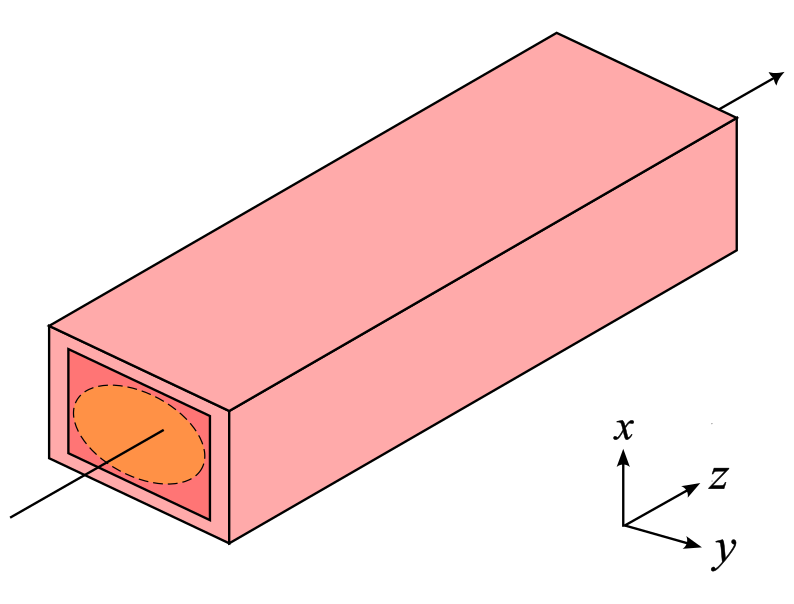
\includegraphics[width=0.6\textwidth]{img/Waveguide schematic diagram.png}
	\caption{波導示意圖與光場傳播方向。}
	\label{fig:waveguide_schematic}
\end{figure}

當波導結構在傳播方向($z$軸)上具備平移對稱性(Translation symmetry)時，我們可以透過將電場進行解分離變數，
寫成沿著$z$方向傳播的形式:
\begin{align}
\vec{E} = \vec{E}(x, y)e^{-i\beta z}
\label{eq:Translation symmetry in Z}
\end{align}

接著將$z$方向傳播形式\eqref{eq:Translation symmetry in Z}帶入亥姆霍茲方程\eqref{eq:helmholtz}後，
對$z$做二次偏微分會得到$-\beta^2$(也就是$\frac{\partial^2}{\partial z^2} \rightarrow -\beta^2$)，
整理後我們可以得到橫截面($xy$平面)上的二維波動方程:
\begin{align}
\left( \frac{\partial^2}{\partial x^2} + \frac{\partial^2}{\partial y^2} \right)\vec{E} + k_0^2 n^2(\vec{r})\vec{E} = \beta^2\vec{E}
\label{eq:xy 2D Wave Equation}
\end{align}

這邊可以定義成一個線性算子(Linear operator)$L$:
\begin{align}
L \triangleq \left( \frac{\partial^2}{\partial x^2} + \frac{\partial^2}{\partial y^2} \right) + k_0^2 n^2(\vec{r})
\label{eq:linear_operator}
\end{align}

因此可以將整個光學波導的模態傳播問題簡化為標準的特徵值問題(Eigenvalue Problem, EVP):
\begin{align}
L\vec{E} = \beta^2\vec{E}
\label{eq:WG Eigenvalue Problem}
\end{align}

在這個式子中，模態(Modes)的空間場分佈就會等於該算子 $L$ 的特徵函數(Eigenfunction)，
而傳播常數的平方 $\beta^2$ 則會等於其對應的特徵值(Eigenvalue)。這個光學特徵值問題在數學形式上，
與量子力學中的一維有限位能井問題(Particle in a box problem)(圖~\ref{fig:Finite Potential Well})有著異曲同工之妙，都必須在邊界條件下求得特定波數與對應的
空間分布，一維定態薛丁格方程(Schrödinger equation)表示如下：
\begin{align}
-\frac{\hbar^2}{2m}\nabla^2\psi + V(\vec{r})\psi = E\psi
\label{eq:1D schrodinger equation}
\end{align}
此式的波函數($\psi$)、位能分布(V($\vec{r}$))與能量特徵值($E$)，分別對應到了波導方程\eqref{eq:xy 2D Wave Equation}中的電場($\vec{E}$)、折射率分布($k_0^2 n^2(\vec{r})$)
以及傳播常數的平方($\beta^2$)。在數學形式的對等性中，我們可以得出光波導兩個核心物理特質的結論:模態量子化(Quantization)與能量侷限性
(Confinement)，只有特定且不連續的$\beta$值才能夠穩定存在於波導中，且折射率的對比愈大，位能井就愈深，則波導對光場的侷限性就越好。\
\begin{figure}[htb]
	\centering
	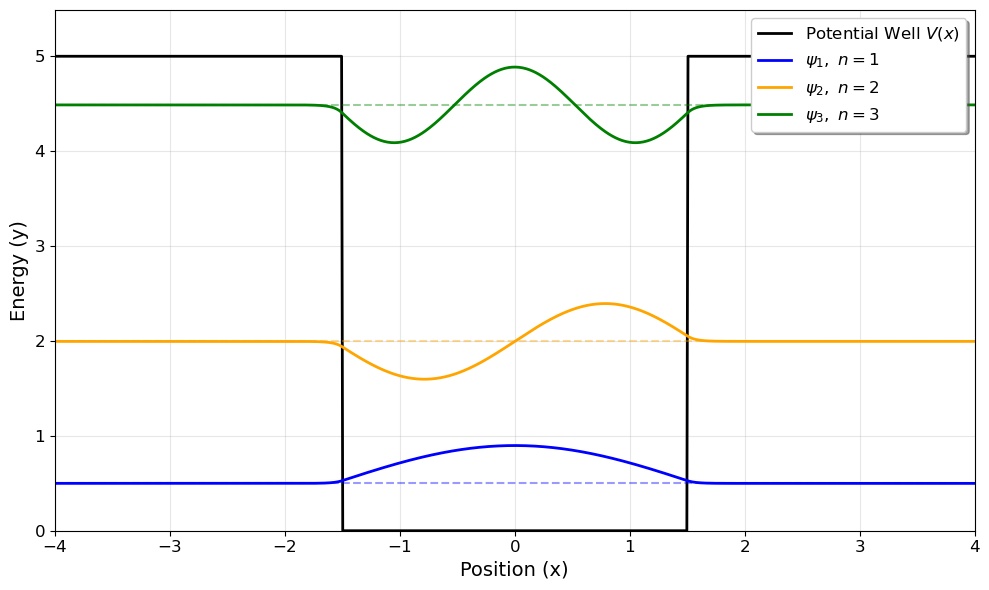
\includegraphics[width=0.9\textwidth]{img/Finite Potential Well.png}
	\caption{一維有限位能井示意圖。}
	\label{fig:Finite Potential Well}
\end{figure}

另外，每個模態的傳播特徵可以由有效折射率(Effective Refractive Index)來定義:
\begin{align}
n_{eff} \triangleq \frac{\beta}{k_0} 
\label{eq:effective refractive index}
\end{align}
因此，對於能夠在波導中穩定傳播的束縛模態，其有效折射率($n_{eff}$)必須介於核心折射率($n_2$)和包層折射率($n_1$)之間，也就是，
\begin{align}
n_{1} < n_{eff} < n_{2}
\label{eq:effective refractive index range}
\end{align}
其原因可由電磁場在核心層與包層中的分布特性來理解。在核心層內，光場必須呈現簡諧波解(Sinusoidal solution)傳播，因此橫向波數需滿足
\begin{align}
h^2\triangleq k_0^2 n_2^2 - \beta^2 > 0
\label{eq:Sinusoidal solution}
\end{align}
由此可得$\beta < n_2 k_0$，也就是$n_{eff} < n_2$。\
另一方面，在包層中光場需以指數衰減的形式向外傳播，也就是漸逝場(Evanescent Field)的形式向外衰減，以確保光能量被侷限於波導內，
因此衰減係數必須滿足
\begin{align}
q^2 = \beta^2 - k_0^2 n_1^2 > 0
\label{eq:Evanescent Field solution}
\end{align}
由此可得$\beta > n_1 k_0$，也就是$n_{eff} > n_1$。
因此，束縛模態的有效折射率必須介於核心層與包層折射率之間，即使是結構較為複雜的反向設計波導，仍然需要滿足以上條件。\

接著，本節參考 A. Yariv 經典光電物理模型中所建立的分析架構 \cite{yariv2007_photonics}，以一維平板波導(Slab Waveguide)結構為例，
考慮只有具備$y$軸分量的橫電模態(Transverse Electric Modes, TE modes)，
其電場可以由以下公式表示:
\begin{align}
E_y(x,z,t)=E_m(x)e^{i(\omega t-\beta z)}
\label{eq:TE mode electric field in slab waveguide}
\end{align}
代入二維波動方程\eqref{eq:xy 2D Wave Equation}可以簡化為一維常微分方程，如下式所示:
\begin{align}
\frac{d^{2}}{d x^{2}}E_{m} + \left[ k_{0}^{2}n^{2}(x) - \beta^{2} \right] E_{m} = 0
\label{eq:TE mode 1D differential equation in slab waveguide}
\end{align}
其中，核心層與包層之折射率分布表示如下:
\begin{align}
n(x) = \begin{cases} n_1, & |x| \ge \frac{d}{2} \\ n_2, & |x| < \frac{d}{2} \end{cases}
\end{align}
由於平板波導的幾何結構在中心軸($x$=0)具有對稱性，因此特徵解可以解為偶對稱(Symmetric)與奇對稱(Anti-Symmetric)的解，
其電場特徵函數 $E_m(x)$ 表示如下：
\begin{itemize}
    \item 偶對稱模態(如TE$_0$, TE$_2$):
    \begin{align}
E_{m}(x) = \begin{cases} C \cos(hx), & |x| < \frac{d}{2} \\ B e^{-q |x|}, & |x| \ge \frac{d}{2} \end{cases}
\label{eq:TE mode symmetric solution}
\end{align}
    \item 奇對稱模態(如TE$_1$, TE$_3$):
    \begin{align}
E_{m}(x) = \begin{cases} C \sin(hx) \cdot \text{sgn}(x), & |x| < \frac{d}{2} \\ B e^{-q |x|} \cdot \text{sgn}(x), & |x| \ge \frac{d}{2} \end{cases}
\label{eq:TE mode anti symmetric solution}
\end{align}
\end{itemize}
此處橫向波數 $h^2 \triangleq k_0^2 n_2^2 - \beta^2 > 0$ 且包層消散係數 $q^2 \triangleq \beta^2 - k_0^2 n_1^2 > 0$ 。\\
根據電磁學邊界條件，在介電質交界面（$x = \pm d/2$）上，切線電場分量 $E_y$ 與切線磁場分量 $H_z$ 皆必須滿足連續條件。
透過法拉第電磁感應定律可導出磁場分量關係式 $H_{z} = \frac{1}{-i\omega\mu}\frac{\partial E_{y}}{\partial x}$ 。
將兩者的電場解代入並應用 $x = d/2$ 處的連續條件，可分別得到對應的齊次線性方程組：
\begin{itemize}
    \item 偶對稱邊界條件:
    \begin{align}
    B e^{-q\frac{d}{2}} - C \cos\left(h\frac{d}{2}\right) &= 0 \\
    B q e^{-q\frac{d}{2}} - C h \sin\left(h\frac{d}{2}\right) &= 0
    \end{align}
    \item 奇對稱邊界條件:
    \begin{align}
    B e^{-q\frac{d}{2}} - C \sin\left(h\frac{d}{2}\right) &= 0 \\
    B q e^{-q\frac{d}{2}} + C h \cos\left(h\frac{d}{2}\right) &= 0
    \end{align}
\end{itemize}
若要使上述方程組存在非平凡解(Nontrivial solutions)，其係數矩陣的行列式值必須嚴格等於零 。
展開行列式並消去共同項 $e^{-qd/2}$ 後，即可成功導出兩種模態的特徵方程式(Characteristic Equations):
\begin{align}
    \begin{aligned}
    \text{Symmetric (偶對稱):} \quad & q = h \tan\left(\frac{hd}{2}\right) \\
    \text{Anti-symmetric (奇對稱):} \quad & q = -h \cot\left(\frac{hd}{2}\right)
    \label{eq:characteristic equations for TE}
    \end{aligned}
\end{align}
將 $h$ 與 $q$ 的定義代回上式\eqref{eq:characteristic equations for TE}，即可得到最終用來求解傳播常數 $\beta$ 的物理關係式:
\begin{align}
    \begin{aligned}
    \text{Symmetric:} \quad & \sqrt{\beta^{2}-{k_{0}}^{2}{n_{1}}^{2}} = \sqrt{k_{0}^{2}n_{2}^{2}-\beta^{2}} \tan\left[\sqrt{k_{0}^{2}n_{2}^{2}-\beta^{2}}\frac{d}{2}\right] \\
    \text{Anti-symmetric:} \quad & \sqrt{\beta^{2}-{k_{0}}^{2}{n_{1}}^{2}} = -\sqrt{k_{0}^{2}n_{2}^{2}-\beta^{2}} \cot\left[\sqrt{k_{0}^{2}n_{2}^{2}-\beta^{2}}\frac{d}{2}\right]
    \label{eq:beta related equations}
    \end{aligned}
\end{align}
在實際的光電工程分析中，此方程式\eqref{eq:beta related equations}可以藉由數值分析工具來進行求解，來計算各階模態精確解的特徵值$\beta$，
以此來描繪出如$\text{TE}_0, \text{TE}_1, \text{TE}_2$等完整模態橫向波函數分佈，如圖~\ref{fig:TE_mode_profile}所示。
\begin{figure}
     \centering
     \begin{subfigure}[]{0.65\textwidth}
         \centering
         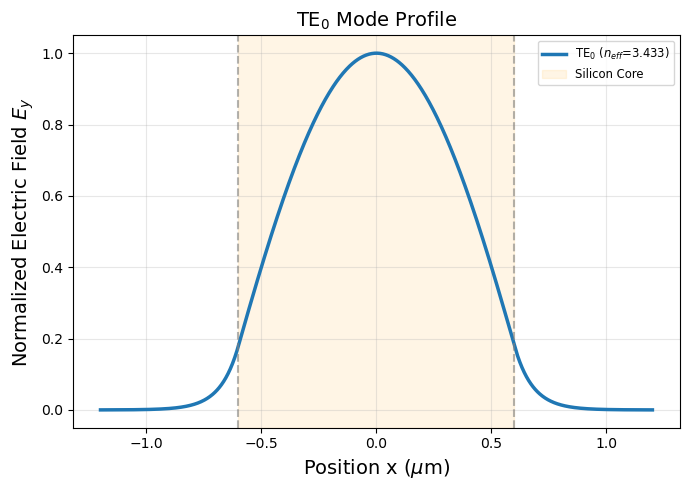
\includegraphics[width=\textwidth]{img/TE0_Profile.png}
         \caption{$\text{TE}_0$ Mode Profile}
         \label{fig:TE0_Profile}
     \end{subfigure}
     \hfill
     \begin{subfigure}[]{0.65\textwidth}
         \centering
         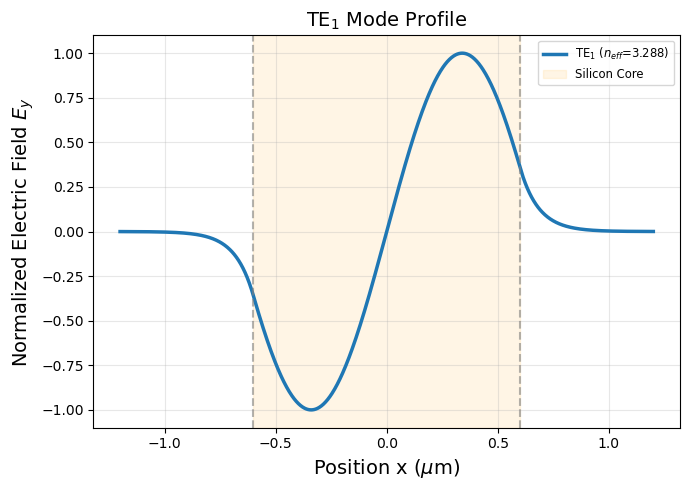
\includegraphics[width=\textwidth]{img/TE1_Profile.png}
         \caption{$\text{TE}_1$ Mode Profile}
         \label{fig:TE1_Profile}
     \end{subfigure}
     \hfill
     \begin{subfigure}[]{0.65\textwidth}
         \centering
         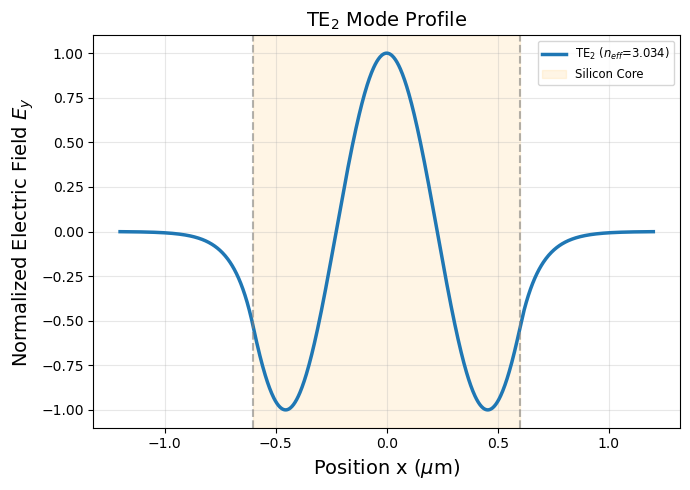
\includegraphics[width=\textwidth]{img/TE2_Profile.png}
         \caption{$\text{TE}_2$ Mode Profile}
         \label{fig:TE2_Profile}
     \end{subfigure}
        \caption{TE$_n$ mode profile for $n=0,1,2$}
        \label{fig:TE_mode_profile}
\end{figure}

%%%%%%%%%%%%%%%%%%%%%%%%%%%%%%%%% 分隔線 %%%%%%%%%%%%%%%%%%%%%%%%%%%%%%%%%%%%%%%%%%%%%%%%%%%
\subsection{Waveguide Discontinuities and Device Principles}

理想直波導具有沿傳播方向($z$ 軸)的平移對稱性，其特徵模態相互正交。然而，矽基光電積體電路(PIC)常需引入彎曲、交叉或多模複合等不連續結構
(Waveguide Discontinuities)以實現光信號路由與多工。這些結構打破了平移對稱性，進而引起散射、輻射及模態間的能量耦合。
本節將分析彎曲波導、交叉波導與模態分波解多工器的物理原理與設計限制。\

\subsubsection{Bend Waveguide}
當光場進入高曲率的 90 度彎曲波導時，等相位面會因曲率而偏轉。為維持波前同步，外側等相位面的相速度須隨半徑線性增加。
當外側相速度超過包層介質的相速度極限（$c/n_{\text{clad}}$ 或 $c/n_1$）時，光場無法滿足全反射條件，從而轉化為散射光場並產生散射損耗。

此空間形變與損耗可藉由 Heiblum 與 Harris 提出的共形映射(Conformal Transformation)理論來描述\cite{heiblum1975_curved_waveguides}。
透過映射函數 $W = u + iv = R \ln(Z/R)$（其中 $Z=x+iy$，$R$ 為等效彎曲半徑），彎曲波導可轉換為 $u,v$ 平面上的等效直波導。
在該坐標系下，波導的等效折射率 $n_{\text{eq}}(u)$ 分佈為：
\begin{align}
n_{\text{eq}}^2(u) = n^2(u) \exp\left(\frac{2u}{R}\right) \approx n^2(u) \left( 1 + \frac{2u}{R} \right)
\label{eq:equivalent refractive index of curved waveguide}
\end{align}
公式顯示，波導外側（$u>0$）的等效折射率隨 $u$ 線性增加，如圖~\ref{fig:bend_waveguide}(b)所示。此折射率梯度使光場中心向外側偏移(Mode Shift)，
導致直波導與彎曲波導銜接時產生模態不匹配損耗(Mode Mismatch Loss)。

利用 WKB 近似(Wentzel-Kramers-Brillouin Approximation)求解此等效模型，可推導出彎曲波導的散射損耗衰減常數 $\alpha$。
在微擾近似下，$\alpha$ 主要由穿透轉折點(Turning Point，即 $n_{\text{eq}}(u) = n_{\text{eff}}$，如圖~\ref{fig:bend_waveguide}(b))外側之勢壘決定，
其正比關係可近似為：

\begin{align}
\alpha \propto \exp\left(-\frac{4\pi}{\lambda_0} R n_{\text{clad}} \delta\right)
\label{eq:radiation loss of curved waveguide}
\end{align}
為了提高$\text{TE}_0$模態的耦合效率，傳統設計通常會採用向外平移（Outward Offset, $\Delta x$，如圖~\ref{fig:bend_waveguide}(a)）技術來對齊銜接處的場型中心。
而當元件尺寸為了提高集成度而大幅縮小時，彎曲半徑 $R$ 的減小會導致散射損耗 $\alpha$ 指數型激增。
此時，傳統的固定半徑與線性平移設計已無法有效兼顧散射損耗與模態不匹配。
因此，本研究採用反向設計方法，對彎曲波導的幾何邊界進行非對稱的結構優化，以突破傳統結構的設計瓶頸。

如圖~\ref{fig:bend_waveguide}所示，(a) 實體空間中，彎曲波導的模態中心向外側偏移，而直、彎波導銜接處可以利用向外平移的方式來對齊光場中心；
(b) 共形映射後，等效直角坐標 $u$ 下的折射率與模態場 $\psi(u)$ 分佈。等效折射率 $n_{\text{eq}}(u)$ 隨空間往外側增加，
在轉折點(Turning Point, $n_{\text{eq}} = n_{\text{eff}}$)外側，光場轉化為振盪的輻射模並造成散射損耗。

\begin{figure}[htbp]
    \centering
    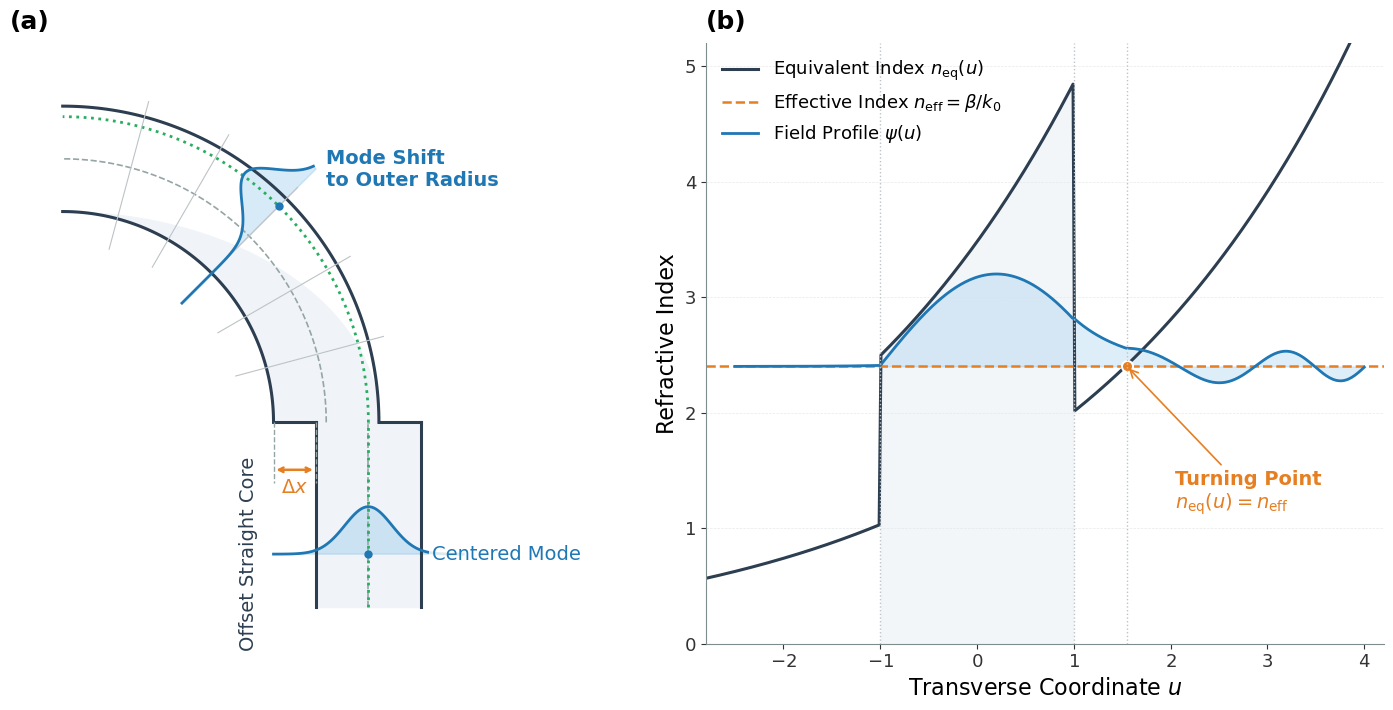
\includegraphics[width=0.95\textwidth]{img/bend_wavegidue.png}
    \caption{彎曲波導中的模態偏移與共形映射分析。}
    \label{fig:bend_waveguide}
\end{figure}

\subsubsection{Waveguide Crossing}
在交叉波導(Waveguide Crossing)結構中，幾何不連續性主要發生於十字交會處。當原本被束縛在輸入波導的特徵模態進入波導交叉處時，
會因為瞬間失去了側邊高折射率差的約束，而光場會衰減為在均勻介質中傳播的自由空間波(Free-space wave)，
進而遵循惠更斯-菲涅耳原理(Huygens–Fresnel Principle)，產生明顯的繞射與發散。

當發散的光場抵達輸出端時，傳輸效率 $\eta$ 在數學上受限於輸入發散場 $\vec{E}_{\text{in}}$ 
與輸出波導特徵模態 $\vec{E}_{\text{out}}$ 之間的重疊積分(Overlap integral)\cite{chrostowski2015_silicon_photonics}:
\begin{align}
\eta = \frac{\left| \iint \vec{E}_{\text{in}} \times \vec{H}_{\text{out}}^* \cdot \hat{z} \, dx dy \right|^2}{\iint \text{Re}(\vec{E}_{\text{in}} \times \vec{H}_{\text{in}}^*) \cdot \hat{z} \, dx dy \iint \text{Re}(\vec{E}_{\text{out}} \times \vec{H}_{\text{out}}^*) \cdot \hat{z} \, dx dy}
\label{eq:overlap_integral}
\end{align}

沒有約束的繞射效應會使輸入場 $\vec{E}_{\text{in}}$ 在空間中快速的發散，而導致上述重疊積分大幅下降，成為元件插入損耗(Insertion Loss)的主因。

這些未與輸出特徵模態匹配的雜散光場，除了部分向基板與包層發散外，大部分會直接散射並耦合至垂直的交叉通道。
這種能量洩漏會導致通道間串擾(Crosstalk)與訊號交叉污染，進而降低積體光學系統的訊號雜訊比(Signal-to-Noise Ratio, SNR)與雜訊容限(Noise Margin)。\

\subsubsection{Mode Division Demultiplexer (DEMUX)}
模態分波解多工器(Mode Division Demultiplexer, DEMUX)用於將單一多模通道中同時傳輸的不同階模態(如 $\text{TE}_0$ 與 $\text{TE}_1$)分離，
並轉換為對應單模輸出通道的基模。根據勞倫茲互易定理(Lorentz Reciprocity)，光的傳播具有可逆性，
因此模態分波多工器(MUX)與解多工器(DEMUX)在物理結構上完全相同，只有傳播方向相反。

在理想的直波導中，各階模態構成完備且正交(Orthogonal)的基底，模態能量互不干擾。若要使特定高階模態發生空間轉移與轉換，
解多工器就必須引入非對稱幾何邊界或拓撲突變。這些細小破碎的結構微擾會打破原有的系統對稱性，使原本的正交性失效。
這種模態轉換與非預期的能量耦合可以用耦合模態理論(Coupled Mode Theory, CMT)\cite{yariv2007_photonics}分析。
假設多模波導中的高階模態為 $a$(傳播常數為 $\beta_a$)，目標單模波導中的基模為 $b$(傳播常數為 $\beta_b$)，
則兩通道間的能量轉移滿足以下耦合微分方程：
\begin{align}
\frac{dA(z)}{dz} &= -i \kappa_{ab} B(z) e^{i\Delta\beta z} \\
\frac{dB(z)}{dz} &= -i \kappa_{ba} A(z) e^{-i\Delta\beta z}
\label{eq:mode coupling of directional coupler}
\end{align}
其中，$A(z)$ 與 $B(z)$ 分別為兩模態沿傳播方向的包絡(Envelope)，相位失配量定義為 $\Delta\beta = \beta_a - \beta_b$。

若要使能量完全轉移，必須滿足相位匹配條件(Phase Matching, $\Delta\beta = 0$)。在此基礎上，引入非對稱幾何微擾 $\Delta \epsilon(x,y)$ 後，
模態間的交叉耦合係數(Cross-coupling coefficient) \cite{yariv2007_photonics}$\kappa_{ab}$可表示為微擾區域的重疊積分：
\begin{align}
\kappa_{ab} = \frac{\omega}{4} \iint \Delta \epsilon(x,y) \vec{E}_a^* \cdot \vec{E}_b \, dx dy
\label{eq:mode cross coupling coefficient}
\end{align}
傳統非對稱的直接耦合器受限於簡單的幾何漸變，容易產生非理想的物理效應。當解多工器引入拓撲突變時，
非預期的能量耦合會隨之增強。若非目標模態在微擾區域內的耦合係數 $\kappa_{mn}$ 不為零，
部分能量會洩漏到其他分離通道，造成通道間的串擾(Crosstalk, CT)。其串擾定義為：
\begin{align}
\text{CT (dB)} = 10 \log_{10} \left( \frac{P_{\text{leakage}}}{P_{\text{target}}} \right)
\label{eq:crosstalk}
\end{align}
其中 $P_{\text{leakage}}$ 為洩漏功率，$P_{\text{target}}$ 為目標通道功率。

此外，元件的插入損耗 (Insertion Loss, IL) 用以描述輸入光功率與目標輸出通道功率之間的損失，其定義為
\begin{align}
\text{IL (dB)} = -10 \log_{10} \left( \frac{P_{\text{target}}}{P_{\text{in}}} \right)
\label{eq:insertion loss}
\end{align}
其中 $P_{\mathrm{in}}$ 為輸入光功率。插入損耗愈小，表示元件的能量傳輸效率愈高。
高串擾會降低系統的訊號雜訊比(Signal-to-Noise Ratio, SNR)，而未成功耦合到目標通道的能量則會增加元件的插入損耗。

因此，由於模態解多工器具有複雜且微細的幾何特徵，且各結構參數對光場分佈與模態耦合存在高度非線性的交互作用，難以透過傳統參數掃描或經驗法則進行設計。
為此，本研究採用反向設計(Inverse Design)方法，利用最佳化演算法在龐大的設計空間中自動搜尋符合性能需求的結構。

\subsection{Finite-Difference Time-Domain (FDTD) Method}

本篇論文所使用的光學模擬方法為MEEP(MIT Electromagnetic Equation Propagation)，是由MIT麻省理工學院的研究團隊於2006年開發的
開源電磁模擬軟體，其方法基於有限差分時域法(Finite-Difference Time-Domain, FDTD)。
本章節內容主要參考其研究團隊於2010年發表的論文\cite{oskooi2010_meep}以及其官方網站的說明\cite{meep_docs}

\subsubsection{Units and Yee Lattice}
在MEEP中，所有物理量皆採用無因次單位(Dimensionless Units)，將基礎物理常數設定為$\epsilon_0 = 1$、$\mu_0 = 1$以及光速$c = 1$。
在此單位制下，馬克士威旋度方程(Maxwell's Curl Equations)化為無因次形式:
\begin{align}
\nabla \times E &= -\frac{\partial H}{\partial t}
\label{eq:maxwell_curl_1}
\end{align}
\begin{align}
\nabla \times H = \varepsilon_{r}(r) \frac{\partial E}{\partial t}
\label{eq:maxwell_curl_2}
\end{align}
其中$\varepsilon_{r}(r)$為相對介電常數。這種單位制的直接結果是：當空間幾何結構與工作波長等比例縮放時，電磁響應完全不變，即馬克士威方程的尺度不變性(Scale Invariance)。
實際應用中，使用者可自定義一個特徵長度單位$a$，其他物理量單位由$a$與$c$推導得出，對應關係如下表所示:
\begin{table}[H] 
\centering
\begin{tabularx}{\textwidth}{c | c | >{\centering\linespread{1.0}\selectfont\arraybackslash}X}
\hline \rule{0pt}{1.8em}
\textbf{物理量 (Physical Quantity)} & \textbf{MEEP 單位表示} & \textbf{實際物理單位 ($a=1\,\mu\text{m}$)} \\ \hline \rule{0pt}{1.5em}
長度 (Length, $L$) & $a$ & $1\,\mu\text{m}$ \\ \hline \rule{0pt}{1.5em}
時間 (Time, $T$) & $a/c$ & $3.33\text{ fs}$ \\ \hline \rule{0pt}{1.5em}
頻率 (Frequency, $f$) & $c/a$ & $300\text{ THz}$ \\ \hline \rule{0pt}{1.5em}
波長 (Wavelength, $\lambda$) & $a/f_{\text{MEEP}}$ & $\lambda = 1/f_{\text{MEEP}}$ \\ \hline
\end{tabularx}
\captionsetup{name=TABLE, font={color=blue, sf, footnotesize}}
\caption{MEEP unit system and practical physical unit examples.}
\label{tab:meep_units}
\end{table}
\noindent 例如，MEEP中設定頻率$f_{\text{MEEP}} = 0.5$時，對應的實際工作波長為$\lambda = a / 0.5 = 2a$。

空間離散化方面，MEEP採用Yee晶格(Yee Grid)技術。如圖~\ref{fig:3D_YEE_Lattice}所示，
Yee晶格的核心做法是將電場$E$與磁場$H$的空間分量在網格中錯開半個步長($\Delta/2$)交替排列。
以三維網格點 $(i, j, k)$ 為基準，各場分量的取樣位置具有嚴格的幾何對稱性：電場分量位於棱
邊中心，例如 $E_x$ 位於 $(i+1/2, j, k)$；磁場分量則位於面中心，例如頂面的磁場分量 $H_z$ 位於 $(i+1/2, j+1/2, k+1)$。
這種交錯排布使得空間偏導數可以用中心差分(Central-difference)近似，具有二階精確度，可有效降低數值色散誤差。
以頂面最前側棱邊的電場 $E_x(i+1/2, j, k+1)$ 位置為例，這邊的 $\partial H_z / \partial y$ 空間偏導數可近似表示為：
\begin{align}
\left.\frac{\partial H_z}{\partial y}\right|_{(i+1/2, j, k+1)} \approx \frac{H_z(i+1/2, j+1/2, k+1) - H_z(i+1/2, j-1/2, k+1)}{\Delta y}
\label{eq:yee_lattice}
\end{align}
\clearpage

\begin{figure}[htb]
	\centering
	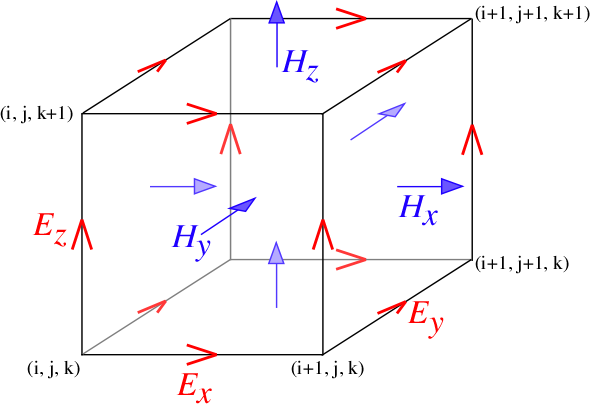
\includegraphics[width=0.6\textwidth]{img/3D_YEE_Lattice.png}
	\caption{三維 Yee 晶格空間分量示意圖\cite{meep_docs}。}
	\label{fig:3D_YEE_Lattice}
\end{figure}

\noindent 本研究之元件數值模擬主要採用二維結構，假設幾何結構在 $z$ 軸無限延伸($\partial / \partial z = 0$)。
在此假設下，馬克士威旋度方程可化簡為兩組對應 TE 與 TM 偏振的方程式。
\begin{itemize}
    \item TE 模態(Transverse Electric)：包含場分量$E_x$、$E_y$與$H_z$，方程式簡化為：
    \begin{align}
    \frac{\partial E_y}{\partial x} - \frac{\partial E_x}{\partial y} = -\frac{\partial H_z}{\partial t}
    \label{eq: E_y}
    \end{align}
    \begin{align}
    \frac{\partial H_z}{\partial y} = \varepsilon \frac{\partial E_x}{\partial t}, \quad -\frac{\partial H_z}{\partial x} = \varepsilon \frac{\partial E_y}{\partial t}
    \label{eq: H_z}
    \end{align}
    \item TM 模態(Transverse Magnetic)：包含場分量$H_x$、$H_y$與$E_z$，方程式簡化為：
    \begin{align}
    \frac{\partial H_y}{\partial x} - \frac{\partial H_x}{\partial y} = \varepsilon \frac{\partial E_z}{\partial t}
    \label{eq: H_y}
    \end{align}
    \begin{align}
    \frac{\partial E_z}{\partial y} = -\frac{\partial H_x}{\partial t}, \quad -\frac{\partial E_z}{\partial x} = -\frac{\partial H_y}{\partial t}
    \label{eq: E_z}
    \end{align}
\end{itemize}
上述方程映射回二維的 Yee 晶格時，三維網格可簡化為 $xy$ 平面上的二維網格。以本研究反向設計之光學模擬所涉及的 TE 模態為例，其二維 Yee 晶格分量配置如圖~\ref{fig:2D_YEE_Lattice} 所示。
在二維網格點 $(i, j)$ 的標準下:
\begin{itemize}
    \item 磁場分量 $H_z$ 位於網格胞體(Cell)之中心點，位置為 $(i+1/2, j+1/2)$。
    \item 電場分量 $E_x$ 與 $E_y$ 則分別位於網格的水平與垂直棱邊中點，位置分別為 $(i+1/2, j)$ 與 $(i, j+1/2)$。
\end{itemize}
藉由這種二維交錯排列，在公式\eqref{eq: H_z} 中計算 $E_x$ 更新所需的 $\partial H_z / \partial y$ 空間偏導數，在網格點 $(i+1/2, j)$ 處可以精確的離散化為：
\begin{align}
\left.\frac{\partial H_z}{\partial y}\right|_{(i+1/2, j)} \approx \frac{H_z(i+1/2, j+1/2) - H_z(i+1/2, j-1/2)}{\Delta y}
\label{eq:yee_lattice_2d}
\end{align}
上述的偏振分離與二維離散化特性，可以減少二維模擬中的記憶體使用和計算成本

\begin{figure}[htb]
\centering
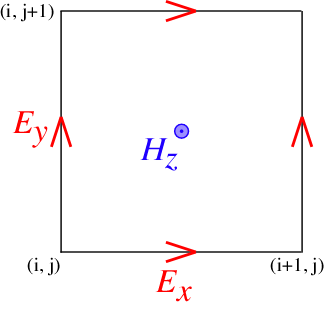
\includegraphics[width=0.45\textwidth]{img/2D_YEE_Lattice.png}
\caption{二維 Yee 晶格空間分量示意圖\cite{meep_docs}。}
\label{fig:2D_YEE_Lattice}
\end{figure}
\clearpage

\subsubsection{Leapfrog Scheme and Courant Condition}
除了在空間上使用 Yee 晶格進行交錯排列外，FDTD 方法在時間軸上也採用了這種類似的交錯取樣策略，稱為跳蛙法(Leapfrog Scheme)。
如圖~\ref{fig:Leapfrog} 所示，電場 $E$ 取在整數時間的步長 $t = n\Delta t$ 進行取樣（如 $E^n, E^{n+1}$），
而磁場 $H$ 則是取在半整數時間的步長 $t = (n+1/2)\Delta t$ 進行取樣（如 $H^{n-1/2}, H^{n+1/2}$）。
\begin{figure}[htb]
\centering
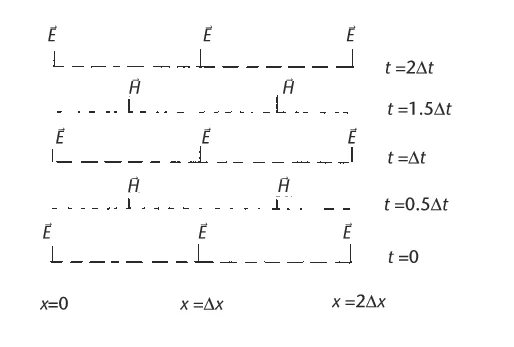
\includegraphics[width=0.45\textwidth]{img/leapfrog.png}
\caption{跳蛙法時間軸示意圖\cite{hao2008fdtd}。}
\label{fig:Leapfrog}
\end{figure}

藉由錯開在時間軸上的半步長，使得馬克士威方程中的時間偏導數都能夠以二階精確度的中心差分進行近似計算。以二維 TE 模態中的公式\eqref{eq: H_z}為例，
電場 $E_x$ 在時間 $t = (n+1/2)\Delta t$ 的時間偏導數可利用中心差分近似為：
\begin{align}
\left.\frac{\partial E_x}{\partial t}\right|^{n+1/2}_{(i+1/2, j)} \approx \frac{E_x^{n+1}(i+1/2, j) - E_x^n(i+1/2, j)}{\Delta t}
\label{eq:leapfrog_time}
\end{align}

將公式\eqref{eq:yee_lattice_2d} 與公式\eqref{eq:leapfrog_time} 代回原方程式\eqref{eq: H_z}，
就可以推導出電場在未來時間步長 $n+1$ 的顯式更新方程式(Explicit Update Equation)，在更新位置 $(i+\frac12,j)$ 處，電場更新方程式可簡寫為:
\begin{align}
E_x^{n+1} = E_x^{n} + \frac{\Delta t}{\varepsilon_r\Delta y} \left( H_{z,j+\frac12}^{\,n+\frac12} - H_{z,j-\frac12}^{\,n+\frac12} \right)
\label{eq:Explicit Update Equation}
\end{align}
由於每一步更新皆直接利用前一時刻已知的場值，因此 FDTD 屬於顯式(explicit)時間積分方法。

同理，磁場 $H_z^{n+1/2}$ 也可以藉由前一個時間步長的磁場與更新時間步長之電場的空間差分計算得到。
這種藉由時間更新迴圈（$E^n \rightarrow H^{n+1/2} \rightarrow E^{n+1}$）在時域中交替迭代的方法，
就是FDTD方法的核心。

然而，在顯式時間迭代過程中，空間網格步長（$\Delta x, \Delta y$）與時間步長（$\Delta t$）並不能任意設定。
為了確保數值解於時間迭代過程中保持穩定，避免產生非物理性的數值發散，時間步長必須根據空間離散的尺度來滿足 Courant-Friedrichs-Lewy(CFL)穩定性條件。
在一般的 $d$ 維空間中，該數值穩定性條件要求：
\begin{align}
\Delta t \le \frac{1}{c \sqrt{ \sum_{m=1}^{d} \frac{1}{\Delta x_m^2} }}
\label{eq:cfl}
\end{align}
在 MEEP 採用的無因次單位制中，光速已設定為 $c = 1$。若假設模擬採用均勻的二維網格（$\Delta x = \Delta y = \Delta$），則公式\eqref{eq:cfl} 可化簡為：
\begin{align}
\Delta t \le \frac{\Delta}{\sqrt{2}} \approx 0.707 \Delta
\end{align}
在實際應用中，MEEP 預設引用一個無因次的 Courant 因子(Courant Factor) $S$，定義為 $S = \Delta t / \Delta$。
MEEP 預設將其保守地設定為 $S = 0.5$（滿足小於 $0.707$ 之要求），以此來提供一般光學模擬足夠的數值穩定性。




\subsubsection{Subpixel Smoothing}

\subsubsection{Perfectly Matched Layer, PML}

\subsubsection{Discrete Fourier Transform (DFT) and Mode Expansion}